\documentclass{beamer}

%packages:
% \usepackage{tfrupee}
% \usepackage{amsmath}
% \usepackage{amssymb}
% \usepackage{gensymb}
% \usepackage{txfonts}

% \def\inputGnumericTable{}

% \usepackage[latin1]{inputenc}                                 
% \usepackage{color}                                            
% \usepackage{array}                                            
% \usepackage{longtable}                                        
% \usepackage{calc}                                             
% \usepackage{multirow}                                         
% \usepackage{hhline}                                           
% \usepackage{ifthen}
% \usepackage{caption} 
% \captionsetup[table]{skip=3pt}  
% \providecommand{\pr}[1]{\ensuremath{\Pr\left(#1\right)}}
% \providecommand{\cbrak}[1]{\ensuremath{\left\{#1\right\}}}
% %\renewcommand{\thefigure}{\arabic{table}}
% \renewcommand{\thetable}{\arabic{table}}      

\setbeamertemplate{caption}[numbered]{}

\usepackage{enumitem}
\usepackage{tfrupee}
\usepackage{amsmath}
\usepackage{amssymb}
\usepackage{graphicx}
\usepackage{txfonts}

\def\inputGnumericTable{}

\usepackage[latin1]{inputenc}                                 
\usepackage{color}                                            
\usepackage{array}                                            
\usepackage{longtable}                                        
\usepackage{calc}                                             
\usepackage{multirow}                                         
\usepackage{hhline}                                           
\usepackage{ifthen}
\usepackage{caption} 
\captionsetup[table]{skip=3pt}  
\providecommand{\pr}[1]{\ensuremath{\Pr\left(#1\right)}}
\providecommand{\cbrak}[1]{\ensuremath{\left\{#1\right\}}}
\renewcommand{\thefigure}{\arabic{table}}
\renewcommand{\thetable}{\arabic{table}}   
\newcommand*{\Comb}[2]{{}^{#1}C_{#2}}
\providecommand{\brak}[1]{\ensuremath{\left(#1\right)}}

% Theme choice:
\usetheme{CambridgeUS}

% Title page details: 
\title{Assignment 5} 
\author{Pericherla Pranav Varma\\CS21BTECH11044}
\date{\today}
% \logo{\large \LaTeX{}}


\begin{document}

    % Title page
    \begin{frame}
        \titlepage 
    \end{frame}

    % Outline
    \begin{frame}{Outline}
        \tableofcontents
    \end{frame}

    \section{Question}
    	\begin{frame}{Question}
    	Papoulis Pillai Ch4 Ex 4-21:\\[9pt]
    Find the probability	$P_n(k)$ for $p=0.5,n=10$ and $k=5$ :\\[6pt]
    
    % Add the table of probability here,
 
    \begin{enumerate}[label=(\alph{enumi})]
    		\item By Using Fundamental Theorem.
    		\item By Using DeMoivre-Laplace Theorem.
    \end{enumerate} 
    	\end{frame}
    	
    	\section{Theory}
    	\begin{frame}{Theory}
    	\begin{itemize}
    	\item \textbf{Fundamental Theorem}:\\
    	Suppose a trial is made repeatedly for $'n'$ number of times, where the probability of success is $'p'$ and of failure is $'q'$. Then the probability $\pr{k}$ of the trial being successful for exactly $'k'$ times is given by:
    	\begin{align*}
    	\pr{k} = \Comb{n}{k} \times p^k \times q^{n-k}.
    	\end{align*}
    	\item \textbf{DeMoivre-Laplace Theorem}:\\
    	When n is very large and k is in the $\sqrt{npq}$ neighbourhood of $np$, we can approximate,
	\begin{align*}
	\Comb{n}{k} \times p^k \times q^{n-k} \simeq \frac{1}{\sqrt{2\pi npq}} \cdot e^{\frac{-(k-np)^2}{2npq}}.
	\end{align*}	    	
    	(This approximation is DeMoivre-Laplace Theorem).
    	\end{itemize}
    	\end{frame}
    	
    \section{Solution}
        \begin{frame}{Solution(a)}
       (a) Substituting given values,\\ $n=10$ , $k=5$ , $p=0.5$ and $q=1-p=0.5$ in Fundamental Theorem,\\[9pt]
         \begin{align*}
         \pr{5} &= \Comb{10}{5} \cdot (0.5)^5 \cdot (0.5)^5 \\
         \pr{5} &= \dfrac{10!}{5!5!} \cdot (\dfrac{1}{2})^{10}\\
         \pr{5} &= 0.246.
         \end{align*}
         Calculating np and npq:
         \begin{align*}
         np &= 10 \cdot \dfrac{1}{2}=5\\
         npq &= 10 \cdot \dfrac{1}{2} \cdot \dfrac{1}{2} = \dfrac{5}{2}
         \end{align*}
    \end{frame}
    \begin{frame}{Solution (b)}
    (b)Substituting $(np = 5)$ and $(npq = \dfrac{5}{2})$ in DeMoivre-Laplace Theorem,\\[9pt]
    \begin{align*}
    \pr{5} &\simeq \dfrac{1}{\sqrt{2\pi(\frac{5}{2})}} \cdot e^{\dfrac{-(5-5)^2}{2(\frac{5}{2})}} \\
    \pr{5} &\simeq \dfrac{1}{\sqrt{5\pi}}\\
    \pr{5} &\simeq 0.252.
    \end{align*}
    \end{frame}
    \begin{frame}
    \begin{figure}[H]
		\centering
			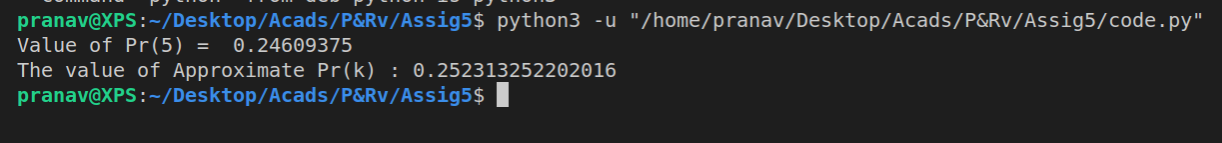
\includegraphics[width=\columnwidth]{figs/output1.png}
			\caption{Verification Code}
			\label{Fig1}	
	\end{figure}
    \end{frame}
\end{document}